\documentclass[10pt]{beamer}
% \setbeamercovered{transparent}
\beamerdefaultoverlayspecification{<+(1)-| alert@+(1)>}
\usetheme{Boadilla}
\usecolortheme{seahorse}
\usefonttheme{structurebold}
\usepackage{multicol}
\usepackage{graphicx}
\usepackage{tikz}
\usepackage{calc}
\usetikzlibrary{calc}
\usepackage{fp}
\usepackage{listings} % Pacote para destacar código fonte
\usepackage{amsmath} 
\usepackage{amssymb} 
\usepackage{helvet}
\usepackage{xcolor}
\usepackage{pgfplots}
\usepackage{array}
\usepackage{arydshln}
\usepackage{enumitem}
\pgfplotsset{compat=1.18}
\setlist[itemize]{label=\textbullet}

\lstset{
  language=C++,
  basicstyle=\small\ttfamily,
  numbers=left, 
  numberstyle=\tiny, 
  stepnumber=1, 
  numbersep=-30pt, 
}

\newcommand{\codecppNoTitle}[2][0.6]{
  \centering
  \begin{minipage}{#1\textwidth}
    %Referencia: https://ctan.dcc.uchile.cl/macros/latex/contrib/listings/listings.pdf
    \lstset{
      language=C++,
      numbers=left,
      numberstyle=\tiny,
      stepnumber=1,
      numbersep=5pt,
      showstringspaces = false,
      frame=shadowbox,
      commentstyle=\color{commentgreen},
      keywordstyle=\color{eminence},
      stringstyle=\color{red},
      backgroundcolor=\color{black!3},
      keywordstyle=\color{blue},
      rulesepcolor=\color{black!5},
      basicstyle=\small\ttfamily, % basic font setting
      emph={int,char,double,float,unsigned,void,bool},
      emphstyle={\color{blue}}
    }
    \lstinputlisting{#2}
  \end{minipage}}


% Definindo as cores para as palavras reservadas
\definecolor{keywordblue}{RGB}{0,0,255}
\definecolor{identifierblack}{RGB}{0,0,0}

\newcommand{\duascolunas}[2]{
  \begin{columns}
    \begin{column}{0.72\textwidth}
      #1
    \end{column}
    \begin{column}{0.28\textwidth}
		#2
	\end{column}
  \end{columns}
}

\title{Análise de Complexidade}
\author{Prof. Kennedy Reurison Lopes}
\subtitle{Parte 2}
\date{\today}

% Início do documento
\begin{document}

\frame{\titlepage}

\begin{frame}
    \frametitle{Cálculo da complexidade}
    Tempo de Execução:
    $$T(n) = \sum^n_{i=1} t_in_i$$
    \begin{itemize}
        \item $i$ índice da instrução;
        \item $t_i$ o tempo necessário para a excução da instrução $i$;
        \item $n_i$ o número de vezes que a instrução $i$ é executada.
    \end{itemize}
\end{frame}

\begin{frame}
    \frametitle{Obtenção de $t_i$}\large
    O cálculo de $t_i$ depende:
    \begin{itemize}
        \item Memória disponível do computador;
        \item Desempenho do processador;
        \item Arquitetura e estado dos dispositivos naquele momento de execução.
    \end{itemize}

    \pause Até mesmo o mesmo computador tem tempo de respostas diferentes.

\end{frame}

\begin{frame}
    \frametitle{Experimento para cálculo do tempo}

    \begin{center}

        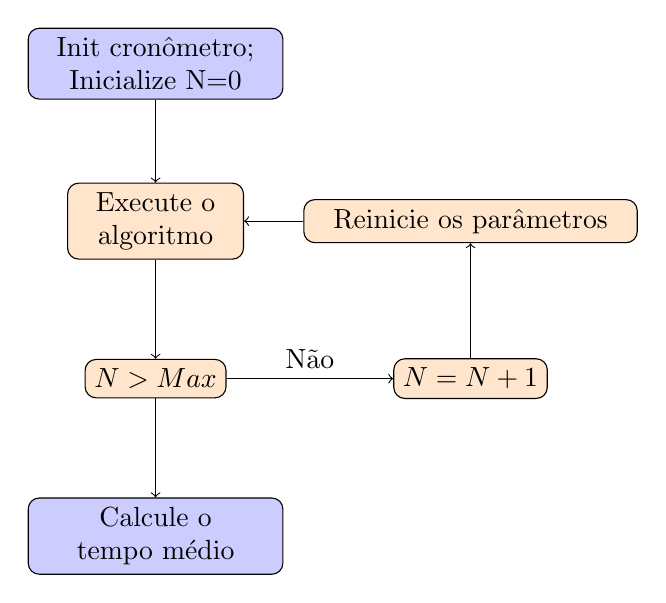
\begin{tikzpicture}[node distance=2cm, every node/.style={rectangle, draw, text centered, rounded corners}]

            % Passo Inicial
            \node<1-> (inicial) [fill=blue!20, rectangle,text width=3cm] {Init cronômetro; Inicialize N=0};

            % Passos Intermediários
            \onslide<2->\node (passo1) [fill=orange!20, below of=inicial, text width=2cm] {Execute o algoritmo};
            \onslide<3->\node (passo2) [fill=orange!20, below of=passo1] {$N>Max$};
            \onslide<6->\node (passo3) [fill=blue!20, below of=passo2,text width=3cm] {Calcule o tempo médio};

            % Conexões
            \onslide<2->\draw [->] (inicial) -- (passo1);
            \onslide<3->\draw [->] (passo1) -- (passo2);
            \onslide<6->\draw [->] (passo2) -- (passo3);

            % Fluxo Alternativo
            \onslide<4->\node (condicao) [fill=orange!20, right of=passo2, node distance=4cm] {$N = N+1$};
            \onslide<5->\node (retorno) [fill=orange!20, above of=condicao, text width=4cm] {Reinicie os parâmetros};

            \onslide<4->\draw [->] (passo2.east) -- node[above, draw=none] {Não} (condicao.west);
            \onslide<5->\draw [->] (condicao.north) -- (retorno.south);
            \onslide<5->\draw [->] (retorno.west) -- (passo1.east);


        \end{tikzpicture}
    \end{center}

\end{frame}

\begin{frame}[fragile, t]
    \frametitle{Contagem de Frequência - Algoritmo 1}

    \begin{lstlisting}[language=C++, basicstyle=\small]
        int main() {
            int x = 0;
            x = x + 1;
            return 0;
        }
  \end{lstlisting}

\end{frame}

\begin{frame}[fragile, t]
    \frametitle{Contagem de Frequência - Algoritmo 2}

    \begin{lstlisting}[language=C++, basicstyle=\small]
        int main() {
            int x = 0, n=10;
            for (int i = 0; i < n; i++) {
                x = x + 1;
            }
            return 0;
        }
  \end{lstlisting}

\end{frame}

\begin{frame}
    \frametitle{Contagem de frequência}
    Exemplo: Conte as operações (contagem de frequência) realizadas na operação de uma soma geométrica definida por:
    $$S = \sum_{i=0}^n x^i$$
    Analise as instruções do algoritmo que o descreve logo a seguir:
\end{frame}

\begin{frame}\normalsize
    \frametitle{Contagem de frequência - Algoritmo 4}
    \duascolunas{\codecppNoTitle[0.9]{algSoma.c}}
    {
        \begin{enumerate}
            \item[L2)] $1$
            \item[L3)] $n+2$
            \item[L4)] $n+1$
            \item[L6)] $\sum_{i=0}^n i$
            \item[L7)] $n+1$
            \item[L9)] $1$
        \end{enumerate}}
    \pause Somando todos os tempos, temos o tempo total:  \begin{center}
        $T(n) = \frac{n^2}{2} + \frac{7n}{2} + 6$
    \end{center}
\end{frame}

\begin{frame}
    \frametitle{Fórmula de \textit{Horner}}

    Pode-se modificar o algoritmo para melhorar o tempo de execução utilizando o algoritmo de \emph{Horner}.
    \begin{align*}
        S = \sum_{i=0}^n x^i & = 1 + x + x^2 +\ldots + x^n                 \\
                             & = 1+x(1 + x + x^2 +\ldots + x^{n-1})        \\
                             & = 1+x(1 + x(1 + x + x^2 +\ldots + x^{n-2})) \\
                             & = 1+x(1+x(1+ x(1+\ldots(1+x(1+x)))\ldots))
    \end{align*}
\end{frame}

\begin{frame}
    \frametitle{Contagem de frequência - Algoritmo 5}
    \duascolunas{\codecppNoTitle[0.9]{algSoma2.c}}{
        \begin{enumerate}
            \pause\item[L2)] 1
                \pause\item [L3)] n+2
                  \pause\item [L4)] n+1
                  \pause\item [L6)] 1
        \end{enumerate}}
    \vfill
    \pause\centering Portanto: $T(n) = 1+(n+2)+(n+1)+1 = 2n+5$.
\end{frame}

\begin{frame}
    \frametitle{Fórmula fechada}
    Uma terceira solução é encontrar a fórmula fechada:
    \begin{align*}
        \onslide<1-> {S = \sum_{i=0}^n i & = 1 + x + x^2 +\ldots + x^n}    \\
        \onslide<2->{xS                  & = x(1 + x + x^2 +\ldots + x^n)} \\
        \onslide<3->{xS                  & = x + x^2 +\ldots + x^{n+1}}    \\
        \onslide<4->{xS +1               & = 1+x + x^2 +\ldots + x^{n+1}}  \\
        \onslide<5->{xS +1               & = S + x^{n+1}}                  \\
        \onslide<6->{xS -S               & = x^{n+1}-1}                    \\
        \onslide<7->{(x-1)S              & = x^{n+1}-1}                    \\
        \onslide<8->{S                   & = \frac{x^{n+1}-1}{x-1}}
    \end{align*}
\end{frame}

\begin{frame}
    \frametitle{Contagem de frequência - Algoritmo 6}
    Qual a complexidade desse algoritmo com a fórmula fechada?\vfill

    \pause\codecppNoTitle[0.9]{algSoma3.c}
    \begin{flushleft}
        \pause Considerando que \emph{pow} tem complexidade logaritmica: $$T(n) = log_2 (n+1)$$
    \end{flushleft}
\end{frame}

\begin{frame}
    \frametitle{Equações }
    \begin{center}

        \begin{tikzpicture}[x=8mm, y=0.7mm]
            % Eixos
            \draw[->,line width=0.25pt] (-1,0) -- (10,0) node[right] {n};
            \draw[->,line width=0.25pt] (1,-10) -- (1,80) node[above] {f(n)};
            \draw[xshift=-14pt] (1,0.1) -- (1,-0.1) node[below] {(1,1)};

            \draw<2->[domain=1:8, smooth=bezier, variable=\x, black,line width=0.5pt]
            plot ({\x},{(\x*\x)/2 + (7*\x)/2 + 6}) node[right] {$\frac{n^2}{2} + \frac{7n}{2} + 6$};
            \draw<3->[domain=1:8, smooth=bezier, variable=\x, black,line width=0.5pt]
            plot ({\x},{2*\x + 5}) node[right, yshift=15] {$2n + 5$};
            \draw<4->[domain=1:8, smooth=bezier, variable=\x, black,line width=0.5pt]
            plot ({\x},{log10(\x+1)}) node[right, yshift=15] {$\log(n+1)$};
        \end{tikzpicture}

    \end{center}
\end{frame}

\newcolumntype{P}[1]{>{\centering\arraybackslash}p{#1}}
\renewcommand{\arraystretch}{1.5}
\begin{frame}
    \frametitle{Comportamento assintótico}
    Comparação numérica da complexidade: Considere que cada operação ($n=1$) dura/custa\footnote{Dura/custa: Termo de comparação dos algoritmos} de $0.0001s = 100\mu s$.\vfill
    \begin{table}[]
        \begin{tabular}{P{2.5cm}P{2.5cm}P{2.5cm}P{2.5cm}}
            $T(n)$      & $20$                 & $40$                       & $60$                                                                                                                         \\ \hline
            $n$         & \only<2->{$200\mu s$ & $400\mu s$                 & $600\mu s$}                                                                                                                  \\ \hdashline
            $n\ log(n)$ & \only<3->{$900\mu s$ & $2.1ms$                    & $3.5ms$}                                                                                                                     \\ \hdashline
            $n^2$       & \only<4->{$4ms$      & $16ms$                     & $36ms$}                                                                                                                      \\ \hdashline
            $n^3$       & \only<5->{$80ms$     & $640ms$                    & $2.16s$}                                                                                                                     \\ \hdashline
            $2^n$       & \only<6->{$10s$      & $27 dias$}   \only<7->{    & $3660$ séculos}                                                                                                              \\ \hdashline
            $3^n$       & \only<8->{$580min$}  & \only<9->{$38550$ séculos} & \only<10->{$1.3*10^{14}$ séculos\footnote{O tempo do universo medido em séculos é de aproximadamente $13.8*10^{7}$ séculos}}
        \end{tabular}
    \end{table}
\end{frame}


\definecolor{olivegreen}{RGB}{85, 107, 47}
\begin{frame}[t]
    \frametitle{Complexidade Assintótica}
    \large O que significa complexidade assintótica?
    \begin{center}
        \begin{tikzpicture}[x=50]
            % Eixo x
            \draw<1->[->, line width=1] (0,0) -- (5,0) node[right] {$n$};
            \draw<1->[->, line width=1] (0,0) -- (0,5) node[above] {$f(n)$};
            \draw<2->[smooth, blue, line width=0.5] plot coordinates {(0,0) (1,1) (2,3) (3,2.5) (4,4) (5,5)};
            \draw<3-6>[smooth, red, line width=0.5] plot coordinates {(0,0) (1,2) (2,2) (3,2) (4,3) (5,3)};
            \draw<4-6>[smooth, olivegreen, line width=0.5] plot coordinates {(0,0) (1,1) (2,3) (3,2) (4,2) (5,2)};
            \draw<7>[smooth, red!20, line width=0.5] plot coordinates {(0,0) (1,2) (2,2) (3,2) (4,3) (5,3)};
            \draw<7>[smooth, olivegreen!20, line width=0.5] plot coordinates {(0,0) (1,1) (2,3) (3,2) (4,2) (5,2)};
            \draw<5>[-, line width=1, dashed] (3,5) -- (3,0) node[below] {$n=3$};
            \draw<6>[-, line width=1, dashed] (2,5) -- (2,0) node[below] {$n=2$};
            \draw<7->[smooth, blue, line width=1.5] plot coordinates {(0,0) (1,1) (2,3) (3,2.5) (4,4) (5,5)};
        \end{tikzpicture}
    \end{center}
\end{frame}

\begin{frame}[t]
    \frametitle{Assíntota}
    \framesubtitle{O que é uma assíntota?}
    São retas horizontais ou verticais que determinam a aproximação das curvas.
    \begin{beamerboxesrounded}{Exemplo}
        \begin{enumerate}[label=\alph*)]
            \setlength\itemsep{1em}
            \item $f(x) = \frac{3x}{x-1}$
            \item $f(x) = \frac{1}{(x-2)^2}$
            \item $f(x) = \frac{(x+2)(x-1)}{x(x+1)(x-2)}$
            \item $f(x) = \frac{x}{\sqrt{x^2+2}}$
            \item $f(x) = 1+e^{-x}$
            \item $f(x) = \log\left(2+3^x\right)$
        \end{enumerate}
    \end{beamerboxesrounded}

\end{frame}

\begin{frame}[t]
    \frametitle{Complexidade Assintótica}
    % \framesubtitle{Notação $O(n)$}
    \begin{beamerboxesrounded}{Definição}
        Uma função $g(n)$ \textbf{domina assintoticamente} outra função f(n) se existem duas constantes positivas $c$ e $m$ tais que, para $n\geq m$, tem-se $$\left|f(n)\right| \leq c\times \left|g(n)\right|$$
    \end{beamerboxesrounded}

    \pause\begin{center}
        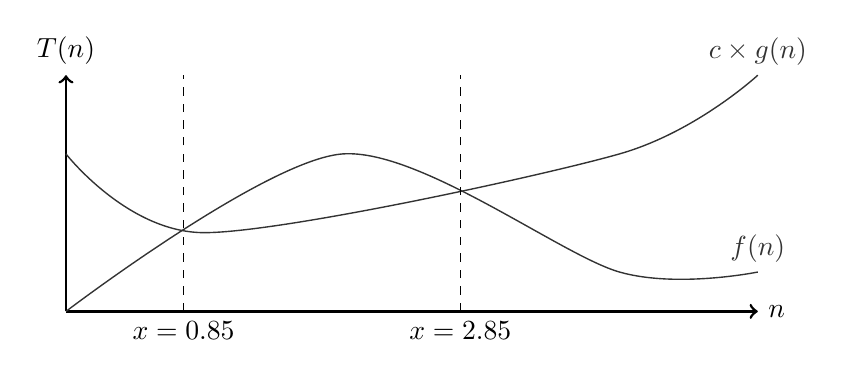
\begin{tikzpicture}[x=50]
            % Eixo x
            \draw[->, line width=1] (0,0) -- (5,0) node[right] {$n$};
            \draw[->, line width=1] (0,0) -- (0,3) node[above] {$T(n)$};
            \draw[smooth, black!80, line width=0.5] plot coordinates {(0,0) (2,2) (4,0.5) (5, 0.5)} node[above] {$f(n)$};
            \draw[smooth, black!80, line width=0.5] plot coordinates {(0,2) (1,1) (4,2) (5, 3)} node[above] {$c\times g(n)$};
            \draw[thin, dashed] (2.85, 0) node[below] {$x=2.85$} -- (2.85, 3);
            \draw[thin, dashed] (0.85, 0) node[below] {$x=0.85$} -- (0.85, 3);
        \end{tikzpicture}
    \end{center}
\end{frame}

\begin{frame}[t]
    \frametitle{Assíntota}
    \framesubtitle{Domínio assintótico}
    \begin{beamerboxesrounded}{Determine quais funções são dominantes:}
        \begin{enumerate}[label=\alph*)]
            \setlength\itemsep{1em}
            \item $f(n)=n$ ou $g(n)=-n^2$
            \item $f(n)=50n$ ou $g(n)=2n^2$
            \item $f(n)=(n+1)^2$ ou $g(n)=n^2$
            \item $f(n)=n^2 + 2n + 1$ ou $g(n)=0.1n^3$
            \item $f(n)=0.2n^2$ ou $g(n)=1000n$
        \end{enumerate}
    \end{beamerboxesrounded}
\end{frame}
\end{document}